\chapter{Praktischer Teil}
\label{sec:praktischerteil}
\begin{onehalfspace}
In diesem Teil der Arbeit werden zuerst die beiden Szenarien erläutert und daraufhin die Konzeption und Umsetzung derer in Python beschrieben.
\section{Szenarien}
\label{subsec:szenarien}
Für das generieren von Daten wurden zwei möglichst reale Szenarien ausgewählt. Zum einen das Szenario eines Bewährungsantrages, für welches 5 verschiedene Attribute und eine endgültige Bewertung mit stattgegeben oder nicht generiert werden. Zum anderen das zweite Szenario des social creditpoint system, für welches pro Person 7 Attribute zu generieren sind und eine numerische Bewertung zwischen 600 und 1400 creditpoints erstellt wird. Diese beiden Szenarien werden im folgenden genauer erläutert.
\subsection{Szenario 1}
\label{subsubsec:szenario1}
In Szenario 1 soll ein Bewährungsantrag einer Person Bewertet werden. Ein Antrag besteht dabei aus dem Namen der Person, dessen Geschlecht, Hautfarbe und den entscheidenden Attributen der laufenden Strafe in Jahre und der Härte des Vergehens. Basierend auf diesen Attributen soll ein Bewerter beurteilen, ob der Antrag genehmigt oder abgelehnt wird. Das Geschlecht wird in \glqq{}Männlich\grqq{} und \glqq{}Weiblich\grqq{} angegeben. Die Hautfarbe der Person wird als \glqq{}Schwarz\grqq{} oder \glqq{}Weiß\grqq{} festgehalten. Die noch laufende Strafe des Gefangenen wird in Jahren von als Ganzzahlen von 1-5 angegeben. Da hier definiert wird ein Bewährungsantrag kann erst ab maximal 5 Jahren noch offene Strafe gestellt werden. Die Härte des Vergehens wird einfachheitshalber in den Gruppen \glqq{}Leicht\grqq{}, \glqq{}Mittel\grqq{} oder \glqq{}Hart\grqq{} festgehalten. \newline
Für die Beurteilung des Antrags von dem Bewerter werden folgende Regeln definiert:
\begin{table}[!h]
    \centering
    \begin{tabular}{|l|l|l|}
    \hline
    \textbf{Attribut}   & \textbf{Positive Auswirkung} & \textbf{Negative Auswirkung} \\ \hline
    Laufende Strafe     & 1-3                          & 4-5                          \\ \hline
    Härte des Vergehens & Leicht, Mittel               & Hart                         \\ \hline
    \end{tabular}
\caption{Tabelle für die Auswirkung der Attributen von Szenario 1}
\label{table:1}
\end{table}\\
Das Geschlecht und die Hautfarbe werden hierbei nicht direkt aufgelistet, da diese in der Regel keine Auswirkung auf die Bewertung haben sollten. Diese können jedoch durch einen konkreten Bias Aussagekraft bekommen. Damit soll in den generierten Daten die gewünschte Verzerrung auf einen gewissen Wert gelegt werden können. In diesem Szenario sind die möglichen Werte, welche durch eine Verzerrung und damit einem menschlichem Vorurteil eines Bewerters beeinflusst werden können, das Geschlecht und die Hautfarbe. Die anderen beiden Attribute, welche in der Tabelle \ref*{table:1} aufgeführt sind, wirken sich durch ihre Ausprägungen positiv oder negativ auf die Bewertung des Antrages aus. So wirkt z.B. eine Härte des Vergehens vom Niveau Leicht sich eher für eine positive Bewertung des Antrages aus, als eine mittlere Härte. Dasselbe gilt auch für die Laufende Strafe. So kann ein Bewerter dann anhand dieser beiden Werte eine Tendenz erhalten und dann über die Gestattung des Antrages entscheiden.
\subsection{Szenario 2}
\label{subsubsec:szenario2}
Im zweiten Szenario wird das durch China populär gewordene sozial creditpoint System in einer lagenunabhängigen Version nachgebaut. Dafür werden Einträge zu Personen erstellt, nach welchen die Punktzahl der einzelnen Person zwischen 600 und 1400 Punkten bestimmt wird. Ein Eintrag zu einer Person beinhaltet die sieben in der folgenden Tabelle dargestellten Attribute mit den unterschiedlichen Ausprägungen.
\begin{table}[!h]
    \centering
    \begin{tabular}{|l|l|}
    \hline
    \textbf{Attribut}       & \textbf{Ausprägungen}                                                                                                \\ \hline
    Name                    & Beliebig                                                                                                             \\ \hline
    Alter                   & 20-79                                                                                                                \\ \hline
    Politische Orientierung & Links, Mitte, Rechts                                                                                                 \\ \hline
    Bildungsabschluss       & \begin{tabular}[c]{@{}l@{}}Ausbildung, Fachschulabschluss, \\ Bachelor, Master, Diplom, Promotion, ohne\end{tabular} \\ \hline
    Soziales                & 0-3                                                                                                                  \\ \hline
    Wohnlage                & \begin{tabular}[c]{@{}l@{}}Großstadt, Kleinstadt,\\ Vorort, Ländlich\end{tabular}                                    \\ \hline
    CO2-Fußabdruck          & 4-12                                                                                                                 \\ \hline
    \end{tabular}
\caption{Tabelle der Attribute und Auswirkungen von Szenario 2}
\label{table:2}
\end{table}
Die in Tabelle \ref*{table:2} aufgeführten Ausprägungen haben ähnlich wie zu Szenario 1 unterschiedlich starke Auswirkungen auf den am Ende bestimmten social Score. Einzig allein der Name und das Alter sollen keine direkte Auswirkung auf den social Score haben. Die anderen Attribute wirken sich je nach Auswirkung positiv durch eine Erhöhung des Scores oder negativ durch eine Verringerung des Scores aus.
Insgesamt werden so in diesem Szenario viele Einträge von Personen erstellt, welche alle unterschiedlichste Verteilungen der Ausprägungen besitzen und dadurch in der Bewertung einen individuellen social Score erzielen. Um nun eine gewünschte Verzerrung in die Daten zu bekommen können alle Attribute bis auf den Namen, welcher rein als Füllwert dient, durch eine Verzerrung beeinflusst werden. So können z.B. Personen zwischen 20-30 Jahre negativ verzerrt werden, da ein oder zwei Bewerter etwas gegen junge Leute haben und diesen aus ihrer Überzeugung einen schlechteren Score geben. In diesem Szenario ist somit eine hohe Variabilität geboten inwieweit eine Verzerrung in die Daten gebracht wird. Zudem kann auch eine Verzerrung über mehrere Attribute eingebracht werden, da ein Bewerter z.B. auch etwas gegen eine Rechte Politische Orientierung und ein schlechtes Soziales Engagement von 0 haben kann. 
\section{Konzeption}
\label{subsection:konzeption}
In diesem Kapitel wird die erarbeitete Konzeption für die Umsetzung der beiden im Kapitel \ref*{subsec:szenarien} aufgeführten Szenarien erläutert. Dabei wird in ein Grobkonzept zur allgemeinen Generierung der Daten und darauf in ein Feinkonzept für jedes Szenario unterteilt.
\subsection{Grobkonzept}
\label{subsubsec:grobkonzept}
Das Grobkonzept beinhaltet die Überlegungen, wie die Programme/Notebooks für die beiden Szenarien generell aufgebaut sein sollen. Der Ablauf der Programme von der Eingabe der Parameter bis hin zu den fertig generierten Daten wird in fünf Schritten durchgeführt. Der Ablauf der Schritte ist in folgendem Programmablaufplan dargestellt.\\
\begin{figure}[h]
    \centering
    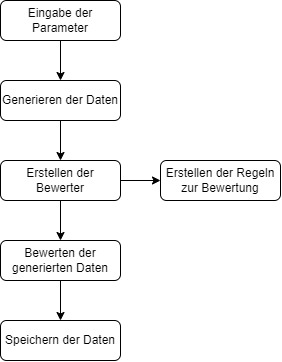
\includegraphics[width=6cm,height=8cm]{Diagramme/Grobkonzept_PAP.jpg}
    \caption{Programmablaufplan der fünf Hauptschritte zur Generierung der Daten}
    \label{fig:GrobkonzeptPAP}
\end{figure}\\
Die in der Abbildung \ref{fig:GrobkonzeptPAP} dargestellten Hauptschritte des Programmablaufs lauten: Parametereingabe, Generieren der Daten, Regeln aufstellen, Bewerten und Speichern der Daten. Im ersten Schritt Parametereingabe wird dem Benutzer die Möglichkeit gegeben die Parameter für die Generierung der Daten einzugeben, wie z.B. die Anzahl der Daten oder Bewerter welche generiert werden sollen. Im folge Schritt werden daraufhin die passende Anzahl an Daten für das jeweilige Szenario generiert. Dabei sollen die Daten möglichst an Verhältnissen aus der Realität angepasst und auf dieser Grundlage generiert werden.
\subsection{Feinkonzept}
\label{subsubsec:feinkonzept}
Hier kommt Feinkonzepte der einzelnen Szenarien.
\section{Umsetzung}
\label{umsetzung}
Hier kommt die Umsetzung der Szenarien mit Code snippets usw.
\newpage
\end{onehalfspace}